% % % % % % % % % % % % % % % % % % % % % % % % % % % % % % % % % % % % % % % % % % % %
%                                                                                     %
% Short Sectioned Assignment LaTeX Template Version 1.0 (5/5/12)                      %
% This template has been downloaded from: http://www.LaTeXTemplates.com               %
%                                                                                     %
% Original author:  Frits Wenneker (http://www.howtotex.com)                          %
%                                                                                     %
% Modified by: Fco Javier Sueza Rodríguez (fcosueza@disroot.org)                      %
%                                                                                     %
% Changes:                                                                            %
%	    - Custom Chapters, Sections and Subsections (titlesec package)                %
%           - Document type scrbook (oneside)                                         %
%           - Use babel-lang-spanish package and marvosym                             %
%           - Use hyperref, enumitem, tcolorbox and glossaries packages               %
%           - Use Time New Roman (mathptmx), Helvetic and Courier fonts               %
%                                                                                     %
% License: CC BY-NC-SA 3.0 (http://creativecommons.org/licenses/by-nc-sa/3.0/)        %
%                                                                                     %
% % % % % % % % % % % % % % % % % % % % % % % % % % % % % % % % % % % % % % % % % % % %

%-----------------------------------------------%
%	              Packages                  %
%-----------------------------------------------%

\documentclass[paper=a4, fontsize=11pt, oneside]{scrbook}

% ---- Text Input/Output ----- %

\usepackage[T1]{fontenc}
\usepackage[utf8]{inputenc}
\usepackage{mathptmx}
\usepackage[scaled=.92]{helvet}
\usepackage{courier}
\usepackage[indent=12pt]{parskip}

\usepackage{geometry}
\geometry{verbose,tmargin=3cm,bmargin=3cm,lmargin=2.6cm,rmargin=2.6cm}

% ---- Language ----- %

\usepackage[spanish]{babel}
\usepackage{marvosym}

% ---- Another packages ---- %

\usepackage{amsmath,amsfonts,amsthm}
\usepackage{graphics,graphicx}
\usepackage{titlesec}
\usepackage{fancyhdr}
\usepackage{tcolorbox}
\usepackage{hyperref}
\usepackage{enumitem}
\usepackage[automake]{glossaries}

%--------------------------------------------------------------------%
%                      Customizing Document                          %
%--------------------------------------------------------------------%


% ----------- Custom Chapters, Sections and Subsections -------------- %

\titleformat{\chapter}[display]
			{\bfseries\Huge}
			{Tema \ \thechapter} {0.5ex}
			{\vspace{1ex}\centering}

\titleformat{\section}[hang]
			{\bfseries\Large}
			{\thesection}{0.5em}{}

\titleformat{\subsection}[hang]
			{\bfseries\large}
			{\thesubsection}{0.5em}{}

\titleformat{\subsubsection}[hang]
			{\bfseries\large}
			{\thesubsubsection}{0.5em}{}

\hypersetup{
    colorlinks=true,
    linkcolor=black,
    urlcolor=magenta
}

% ------------------- Custom heaaders and footers ------------------- %

\pagestyle{fancyplain}

\fancyhead[]{}
\fancyfoot[L]{}
\fancyfoot[C]{}
\fancyfoot[R]{\thepage}

\renewcommand{\headrulewidth}{0pt} % Remove header underlines
\renewcommand{\footrulewidth}{0pt} % Remove footer underlines

\setlength{\headheight}{13.6pt} % Customize the height of the header

% --------- Numbering equations, figures and tables ----------------- %

\numberwithin{equation}{section} % Number equations within sections
\numberwithin{figure}{section} % Number figures within sections
\numberwithin{table}{section} % Number tables within sections

% ------------------------ New Commands ----------------------------- %

\newcommand{\horrule}[1]{\rule{\linewidth}{#1}} % Create horizontal rule command


%----------------------------------------------------------------------------------------
%	TÍTULO Y DATOS DEL ALUMNO
%----------------------------------------------------------------------------------------

\title{
\vspace{10ex}
\normalfont \normalsize
\huge \textbf{Tarea 1: Plataformas de Programación Web en el Entorno Servidor. Aplicaciones LAMP}
}
\author{Francisco Javier Sueza Rodríguez}
\date{\normalsize\today}

%----------------------------------------------------------------------------------------
%                                     DOCUMENTO
%----------------------------------------------------------------------------------------
\begin{document}

\maketitle

\thispagestyle{empty}

\vspace{65ex}

\begin{center}
    \begin{tabular}{l l}
        \textbf{Centro}: & IES Aguadulce \\
        \textbf{Ciclo Formativo}: & Desarrollo Aplicaciones Web (Distancia)\\
        \textbf{Asignatura}: & Desarrollo Web en Entorno Servidor\\
        \textbf{Tema}: & Tema 1 -  Plataformas de Programación Web en el Entorno Servidor.\\
    \end{tabular}
\end{center}

\newpage

\section{Caso Práctico}
La asociación \textbf{Respira} para la atención de menores en situación de riesgo de exclusión social ha recibido una pequeña subvención para el desarrollo de estrategias digitales en el ámbito de su actividad. La asociación tiene su sede central en un barrio conflictivo donde reciben multitud de casos, principalmente de menores y familias en situaciones muy complejas, a los que intentan ayudar con los pocos medios que tienen.

\textbf{Juan} y \textbf{María} han recibido el proyecto con los brazos abiertos y están dispuestos a dar el todo por el todo para que esta asociación ayude a un mayor número de personas. \textbf{María} está especialmente motivada, dado que es el barrio donde ella se crío cuando era pequeña.

\section{Ejercicios}

\subsection{Ejercicio 1}
¿Qué tipo de proyectos podría hacer la asociación \textbf{Respira} con el dinero recibido? Actualmente no tiene web, ¿se te ocurre como podrían mejorar su actividad y su proyección?

\subsubsection{Solución}
Para mejorar su actividad y proyección podrían emplear la subvención recibida para varios proyecto. El principal sería la \textbf{creación de una página web}, que va a ser en el que nos centremos en este ejercicio, pero también podría incluirse la \textbf{creación de puestos informáticos en el centro}, para permitir a los jóvenes que no tengan recursos tener acceso a internet, incluida a la propia página web.

Respecto a la creación de la \textbf{página web}, se podría contratar a un desarrollar web para que creara la aplicación web necesaria. La página, además de la \textbf{información relativa} a todos los \textbf{servicios} que ofrece la asociación, podría tener diversos \textbf{canales de comunicación}.

Por ejemplo, se podría implementar un \textbf{chatbot} para responder a la preguntas frecuentes de forma más inmediata. Además, sería interesante la creación de un \textbf{foro} donde los usuarios pudieran exponer sus dudas sobre cualquier tema relacionado con la asociación, para que estas se pudieran responder y debatir. Siendo además un buen canal para recibir feedback de los usuarios y mejorar, en la medida de lo posible, el funcionamiento de la asociación.

También debería incluir varias \textbf{secciones con información} sobre la asociación así como las diferentes actividades que se realicen, siendo interesante la inclusión de una \textbf{calendario} donde se pueda acceder a la actividades previstas de forma sencilla y rápida.

Esta web proporcionaría \textbf{más visibilidad}, \textbf{mejorando la proyección} de la asociación y permitiendo que los usuarios estén más implicados en esta.

Además de esta web, sería interesan añadir una serie de\textbf{ puestos informáticos}, si el presupuesto lo permite, donde además de acceder a la propia web, permitiera a los usuarios con menos recursos acceder a internet para realizar diferentes gestiones, incluso podría valorarse la creación de algún curso online de inicialización a las nuevas tecnologías, uso de editores de texto, creación de CV, etc...

\subsection{Ejercicio 2}
Fíjate en el siguiente ejemplo que describe la interacción en entre navegador (cliente web) y servidor web donde se detalla lo que ocurre en cada una de las partes. Intenta pensar en otro ``Caso de uso'' donde un potencial usuario (o miembro de la organización) utilice la página web de la asociación Respira para una acción concreta y detalla lo que ocurriría paso por paso.

\begin{figure}[H]
    \begin{tcolorbox}[sharp corners, colback=yellow!30, colframe=white!20]
     \textbf{Caso de Uso: Un voluntario rellena un formulario}
     \vspace{3ex}
     \begin{enumerate}
         \item La persona voluntaria está visualizando un formulario en la página web de la asociación y ha terminado de rellenarlo, con lo que hace clic en ``enviar''.
         \item El navegador realiza una petición tipo HTTP POST al servidor web.
         \item El servidor web recibe la petición con los datos del formulario, y, siguiendo su configuración, detecta que esa petición corresponde a un script PHP y que debe ser redireccionada al motor de ejecución PHP.
         \item El motor PHP (PHP engine) se arranCA e inicia la ejecución del script el cual contiene:
         \begin{enumerate}
             \item Código para comprobar si los datos recibidos son correctos.
             \item Código para almacenar los datos recibidos en la base de datos.
             \item Código para generar HTML con la respuesta al candidato a la candidata.
         \end{enumerate}
         \item Una vez que el motor PHP ha terminado de ejecutar el script, el HTML generado es enviado al servidor web como resultado de la ejecución.
         \item El servidor web recoge el resultado generado por el motor PHP y lo envía al navegador con una respuesta HTTP.
         \item El navegador HTTP recibe la respuesta que incluye el HTML y lo renderiza para que la persona candidata lo vea.
     \end{enumerate}
    \end{tcolorbox}
\end{figure}

\subsubsection{Solución}
El caso de uso que vamos a proponer es el de un usuario que \textbf{realiza una búsqueda en el foro} para que se muestren los mensajes o hilos con una una determinada palabra.

\begin{figure}[H]
    \begin{tcolorbox}[sharp corners, colback=yellow!30, colframe=white!20]
        \textbf{Caso de Uso: Búsqueda de mensajes en el foro}
        \vspace{3ex}
        \begin{enumerate}
            \item El usuario que esta en la página relativa a los foros, introduce un termino en la caja de búsqueda y pulsa en \textbf{\textit{Enviar}}.
            \item El navegador realiza una \textbf{petición tipo HTTP POST} o \textbf{GET}, dependiendo de como se haya programado la página, al servidor.
            \item El \textbf{servidor web} recibe la petición con los datos de la búsqueda, y pasa la petición al \textbf{motor PHP} para que se ejecute el script adecuado.
            \item El \textbf{motor PHP} se inicializa e inicia la ejecución del script el cual contiene:
            \begin{enumerate}
                \item Código para realizar una \textbf{llamada a la base de datos} y obtener todos los mensajes que contengan el termino de búsqueda.
                \item Código para \textbf{filtrar y ordenar el resultado}, para que se muestre de una forma más adecuada al usuario.
                \item Código para \textbf{generar HTML}  y que el resultado se muestre de forma apropiada en la web.
            \end{enumerate}
            \item Una vez que se a \textbf{procesado el script}, el motor PHP pasa el resultado al servidor web, para que este pueda servirlo al cliente.
            \item El \textbf{servidor web} procesa el resultado del motor PHP y lo manda al cliente web.
            \item El \textbf{cliente} recibe el resultado y lo renderiza.
        \end{enumerate}
    \end{tcolorbox}
\end{figure}

\subsection{Ejercicio 3}
Rellena la siguiente tabla indicando casos concretos en los que podría ser necesario emplear las siguientes tecnologías en el desarrollo de la web de la asociación \textbf{Respira}:

    \begin{figure}[H]
    \centering
    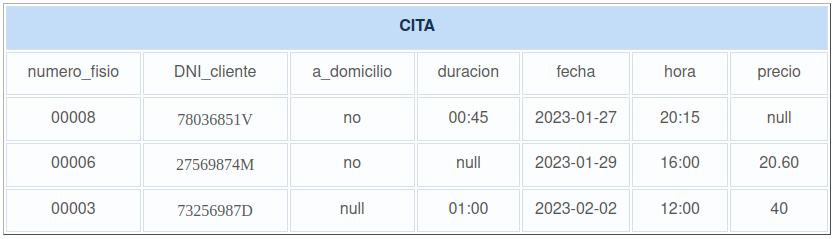
\includegraphics[scale=0.60]{tabla-enunciado.png}
\end{figure}

\subsubsection{Solución}
A continuación se muestra la tabla rellena con la información solicitada.

\begin{figure}[H]
    \centering
    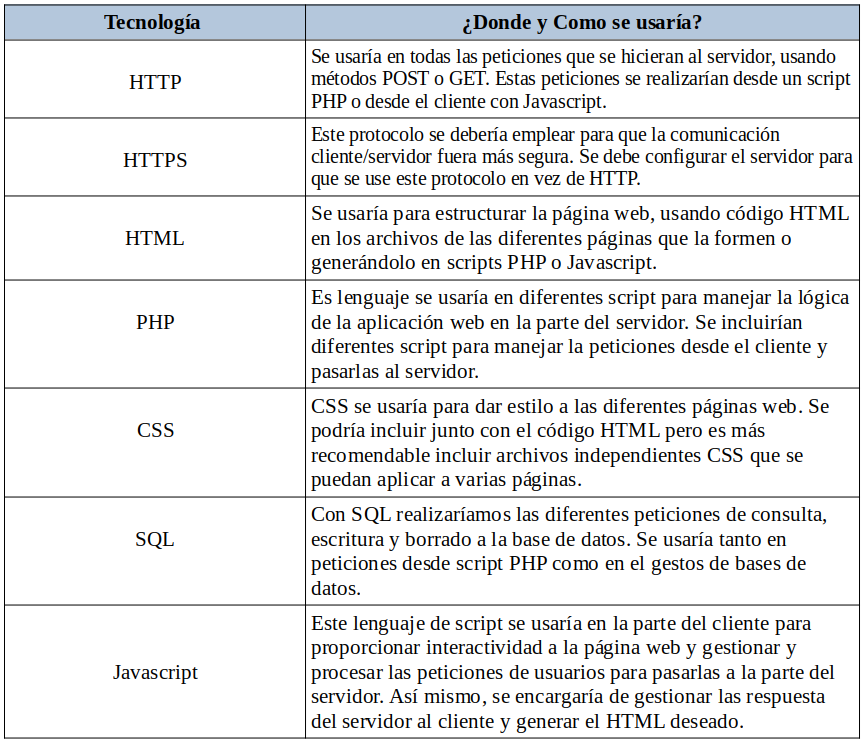
\includegraphics[scale=0.60]{tabla-solucion.png}
\end{figure}

\subsection{Ejercicio 4}
Realiza la instalación de XAMPP 8.2.4 en tu ordenador (preferiblemente en C:/XAMPP) y realiza lo siguiente:

\begin{itemize}
    \item Realiza una captura de pantalla durante el proceso de instalación.
    \item Realiza una captura de pantalla de la interfaz de XAMPP para arrancar o detener el servidor web.
    \item Localiza la carpeta donde podemos añadir nuestras aplicaciones web (generalmente C:/xampp/htdocs) y añade un script llamado phpinfo.php. Añade el siguiente código en su interior: <?php phpinfo(); ?>. Crea una captura de pantalla de lo que aparece en el navegador al acceder a la URL asociada a dicho script (previsiblemente será http://localhost/phpinfo.php).
\end{itemize}

\begin{figure}[H]
    \begin{tcolorbox}[sharp corners, colback=yellow!30, colframe=white!20]
\textbf{NOTA}: hay un error en la numeración de los ejercicios en la página de la tarea, pasando de ejercicio 3 al 5, por lo que en este documento se van a numerar omitiendo ese error, este sería el ejercicio 5 de la descripción de la tarea.
    \end{tcolorbox}
\end{figure}

\subsubsection{Solución}
En este ejercicio se debía realizar la instalación de XAMPP, pero a riesgo de que el ejercicio puntúe como no realizado, \textbf{no he instalado} dicha versión de AMP, ya que durante el proceso de estudio de la asignatura \textbf{se instaló LAMP} en la distribución Linux que uso, una Kubuntu en concreto.

El \textbf{problema }es que me ha costado un poco configurar la instalación, ya que estoy usando virtual hosts en Apache 2 para cada uno de los temas de la asignatura, y la instalación de XAMPP puede ``trastocarme'' la instalación ya realizada.

Así, en lugar de mostrar capturas del proceso de instalación de XAMPP, se mostrarán de los paquetes ya instalados y de los comandos usados para arrancar y detener el servidor web, que se realizan usando systemctl.



% Bibliography

%\newpage
%\bibliography{citas}
%\bibliographystyle{unsrt}

\end{document}